\documentclass[12pt, openany, oneside]{book}

\usepackage{listings}
\usepackage[dvipsnames]{xcolor}
\usepackage{ctex}
\usepackage{fontspec}
\usepackage{setspace}
\usepackage{tikz}
\usepackage{anyfontsize}
\usepackage{sectsty}
\usepackage{titlesec}
\usepackage{float}
\usepackage[hidelinks]{hyperref}
\usepackage[a4paper]{geometry}
\usepackage{url}
\usepackage{amssymb}
\usepackage{fontawesome5}
\usepackage[most]{tcolorbox}
\usepackage{stackengine}
\usepackage{multirow}
\usepackage[T1]{fontenc}
% \usepackage{minted}

\usetikzlibrary{calc,trees,positioning,arrows,fit,shapes}
\usetikzlibrary{shapes.multipart,chains}

\tikzstyle{startend} = [rectangle, rounded corners, minimum width=3cm, minimum height=1cm, text centered, draw=black, fill=red!30]
\tikzstyle{io}        = [trapezium, trapezium left angle=70, trapezium right angle=110, minimum width=3cm, inner xsep = -15pt, minimum height=1cm, text centered, draw=black, fill=blue!30]
\tikzstyle{process}   = [rectangle, minimum width=3cm, minimum height=1cm, inner ysep=0, text centered, draw=black, fill=orange!30]
\tikzstyle{decision}  = [diamond,shape aspect=2.5, minimum width=3cm, minimum height=1cm, inner xsep=0,text centered, draw=black, fill=green!30]
\tikzstyle{arrow}     = [thick,->,>=stealth]

\def\rlwd{.5pt} \def\rlht{2.2ex} \def\rldp{.5ex}
\def\mydiv#1{~%
  \rule[-\rldp]{\rlwd}{\rlht}%
  \setbox0=\hbox{~#1}%
  \stackunder[\dimexpr\rldp-\rlwd]{~#1}{\rule{\wd0}{\rlwd}}%
}

\definecolor{mycolor}{RGB}{0,128,128}
\newtcbox{\mybox} {
    on line,
    colback=mycolor,
    fontupper=\bfseries\color{white},
    boxrule=0pt,
    arc=5pt, 
    boxsep=0pt, 
    left=2pt, 
    right=2pt, 
    top=5pt, 
    bottom=5pt
}

\setstretch{1.5}
\setlength{\parindent}{0cm}

\geometry{a4paper,top=2.5cm,bottom=2.5cm}

\titleformat{\chapter}{\Huge\Huge\bfseries}{\chaptertitlename\ \thechapter{\ }}{0pt}{\Huge}{}
\titlespacing{\chapter}{0pt}{0pt}{12pt}

\definecolor{dkgreen}{rgb}{0,0.4,0}
\definecolor{gray}{rgb}{0.5,0.5,0.5}
\definecolor{mauve}{rgb}{0.58,0,0.82}
\definecolor{LightGray}{gray}{0.9}

\lstset{
    basicstyle=\linespread{1.3} \fontspec{Consolas},    %  the size of the fonts that are used for the code
	basewidth=0.5em,
    numbers=left,            % where to put the line-numbers
    numberstyle=\color{black},  % the style that is used for the line-numbers
    numbersep=10pt,                  % how far the line-numbers are from the code
    backgroundcolor=\color{white},
    showspaces=false,
    showstringspaces=false,
    showtabs=false,
    frame=single,                   % adds a frame around the code
    rulecolor=\color{black},        % if not set, the frame-color may be changed on line-breaks within not-black text (e.g. commens (green here))
    tabsize=4,                      % sets default tabsize to 2 spaces
    captionpos=t,                   % sets the caption-position to bottom
    breaklines=false,                % sets automatic line breaking
    breakatwhitespace=true,        % sets if automatic breaks should only happen at whitespace
    title=\lstname,                   % show the filename of files included with \lstinputlisting;
    % also try caption instead of title
    numberstyle=\color{black},		% line number color
    keywordstyle=\color{blue},          % keyword style
    commentstyle=\color{dkgreen},       % comment style
    stringstyle=\color{mauve},         % string literal style
    escapeinside={\%*}{*)},            % if you want to add LaTeX within your code
    morekeywords={*,...}               % if you want to add more keywords to the set
}

\begin{document}

\pagestyle{plain}

\begin{tikzpicture}[overlay,remember picture]
	% Background color
	\fill[
		black!2]
	(current page.south west) rectangle (current page.north east);

	% Rectangles
	\shade[
		left color=Dandelion,
		right color=Dandelion!40,
		transform canvas ={rotate around ={45:($(current page.north west)+(0,-6)$)}}]
	($(current page.north west)+(0,-6)$) rectangle ++(9,1.5);

	\shade[
		left color=lightgray,
		right color=lightgray!50,
		rounded corners=0.75cm,
		transform canvas ={rotate around ={45:($(current page.north west)+(.5,-10)$)}}]
	($(current page.north west)+(0.5,-10)$) rectangle ++(15,1.5);

	\shade[
		left color=lightgray,
		rounded corners=0.3cm,
		transform canvas ={rotate around ={45:($(current page.north west)+(.5,-10)$)}}] ($(current page.north west)+(1.5,-9.55)$) rectangle ++(7,.6);

	\shade[
		left color=orange!80,
		right color=orange!60,
		rounded corners=0.4cm,
		transform canvas ={rotate around ={45:($(current page.north)+(-1.5,-3)$)}}]
	($(current page.north)+(-1.5,-3)$) rectangle ++(9,0.8);

	\shade[
		left color=red!80,
		right color=red!80,
		rounded corners=0.9cm,
		transform canvas ={rotate around ={45:($(current page.north)+(-3,-8)$)}}] ($(current page.north)+(-3,-8)$) rectangle ++(15,1.8);

	\shade[
		left color=orange,
		right color=Dandelion,
		rounded corners=0.9cm,
		transform canvas ={rotate around ={45:($(current page.north west)+(4,-15.5)$)}}]
	($(current page.north west)+(4,-15.5)$) rectangle ++(30,1.8);

	\shade[
		left color=RoyalBlue,
		right color=Emerald,
		rounded corners=0.75cm,
		transform canvas ={rotate around ={45:($(current page.north west)+(13,-10)$)}}]
	($(current page.north west)+(13,-10)$) rectangle ++(15,1.5);

	\shade[
		left color=lightgray,
		rounded corners=0.3cm,
		transform canvas ={rotate around ={45:($(current page.north west)+(18,-8)$)}}]
	($(current page.north west)+(18,-8)$) rectangle ++(15,0.6);

	\shade[
		left color=lightgray,
		rounded corners=0.4cm,
		transform canvas ={rotate around ={45:($(current page.north west)+(19,-5.65)$)}}]
	($(current page.north west)+(19,-5.65)$) rectangle ++(15,0.8);

	\shade[
		left color=OrangeRed,
		right color=red!80,
		rounded corners=0.6cm,
		transform canvas ={rotate around ={45:($(current page.north west)+(20,-9)$)}}]
	($(current page.north west)+(20,-9)$) rectangle ++(14,1.2);

	% Year
	% \draw[ultra thick,gray]
	% ($(current page.center)+(5,2)$) -- ++(0,-3cm)
	node[
			midway,
			left=0.25cm,
			text width=5cm,
			align=right,
			black!75
		]
		{
			% {\fontsize{25}{30} \selectfont \bf ANNUAL \\[10pt] REPORT}
		}
	node[
			midway,
			right=0.25cm,
			text width=6cm,
			align=left,
			orange]
		{
			% {\fontsize{72}{86.4} \selectfont 2020}
		};

	% Title
	\node[align=center] at ($(current page.center)+(0,-5)$)
	{
	{\fontsize{72}{72} \selectfont {{Java}}} \\[2cm]
	{\fontsize{20}{19.2} \selectfont \textcolor{orange}{ \bf 极夜酱}} \\[4pt]
	};
\end{tikzpicture}

\newpage

\setcounter{tocdepth}{1}
\tableofcontents
\thispagestyle{empty}

\newpage

\setcounter{page}{1}

\chapter{Java简介}

\section{编程简介}

\subsection{编程简介}

程序(program)是为了让计算机执行某些操作或者解决问题而编写的一系列有序指令的集合。由于计算机只能够识别二进制数字0和1,因此需要使用特殊的编程语言来描述如何解决问题过程和方法。\\

算法(algorithm)是可完成特定任务的一系列步骤,算法的计算过程定义明确,通过一些值作为输入并产生一些值作为输出。\\

流程图(flow chart)是算法的一种图形化表示方式,使用一组预定义的符号来说明如何执行特定任务。

\begin{itemize}
	\item 圆角矩形:开始和结束
	\item 矩形:数据处理
	\item 平行四边形:输入/输出
	\item 菱形:分支判断条件
	\item 流程线:步骤
\end{itemize}

\begin{figure}
	\centering
	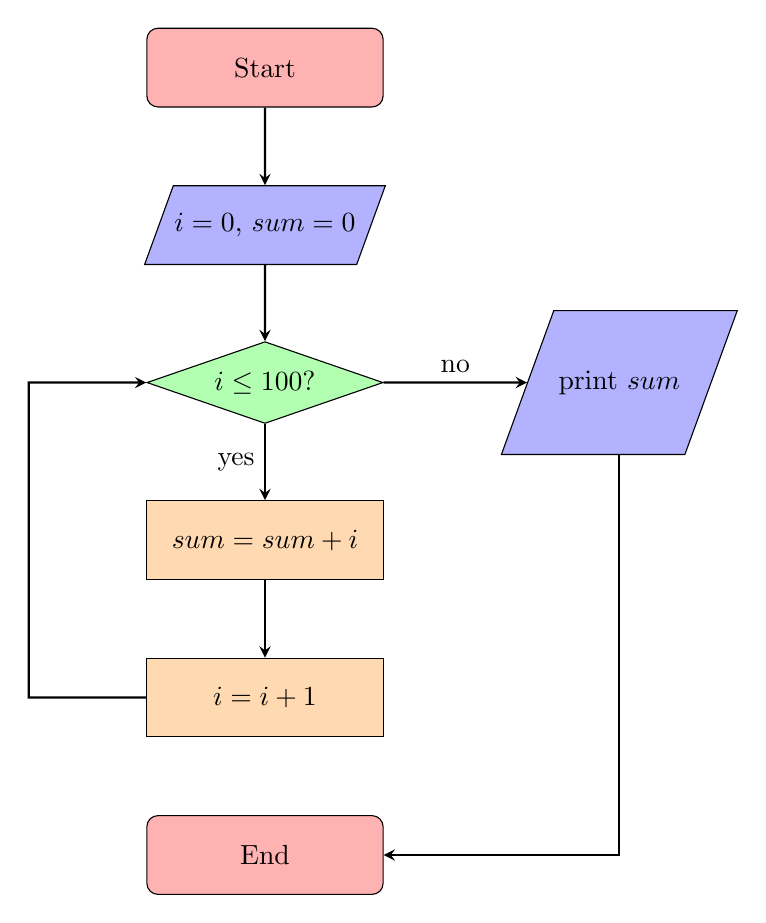
\begin{tikzpicture}[node distance=2cm]
		\node (start) [startend] {Start};
		\node (init)   [io, below of=start] {$ i = 0 $, $ sum = 0 $};
		\node (decision)  [decision, below of=init] {$ i \le 100 $?};
		\node (accumulation) [process, below of=decision] {$ sum = sum + i $};
		\node (update) [process, below of=accumulation] {$ i = i + 1 $};
		\node (output) [io, right of=decision, xshift=2.5cm] {print $ sum $};
		\node (end) [startend, below of=update] {End};

		\draw [arrow] (start) -- (init);
		\draw [arrow] (init) -- (decision);
		\draw [arrow] (decision) -- node[anchor=east] {yes } (accumulation);
		\draw [arrow] (accumulation) -- (update);
		\draw [arrow] (update) -- (-3,-8) -- (-3,-4) -- (decision);
		\draw [arrow] (decision) -- node[anchor=south] {no} (output);
		\draw [arrow] (output) |- (end);
	\end{tikzpicture}
	\caption{计算$ \sum_{i=1}^{100} i $的流程图}
\end{figure}

\vspace{0.5cm}

\subsection{编程语言(Programming Language)}

编程语言主要分为面向机器、面向过程和面向对象三类。C语言是面向过程的语言,常用于操作系统、嵌入式系统、驱动程序、图形引擎、图像处理、声音效果等。\\

Java是面向对象语言,吸收了C/C++的优点,并摒弃了难以理解的多继承、指针等概念。Java可以编写桌面应用程序、Web应用程序、分布式系统和嵌入式系统应用程序等。

\begin{figure}[H]
	\centering
	
\includegraphics[scale=0.9]{img/C1/1-1/1.png}
	\caption{常见编程语言}
\end{figure}

\newpage

\section{Hello World!}

\subsection{Hello World!}

\mybox{Hello World!}

\begin{lstlisting}[language=Java]
public class HelloWorld {
    public static void main(String[] args) {
        System.out.println("Hello World!");
    }
}
\end{lstlisting}

\begin{tcolorbox}
	\mybox{运行结果}
	\begin{verbatim}
Hello World!
	\end{verbatim}
\end{tcolorbox}

第一行语句中的public为访问修饰符,一共有三种:public、private、protected。第一行中class表示一个类,类名需要与文件名相同。\\

第二行中的main()是程序的入口。\\

第三行的语句System.out.println()的作用是在屏幕上输出“Hello World”这个字符串。【;】表示语句结束,注意不要使用中文的分号。\\

\subsection{字节码文件}

Java编译器(compiler)的作用是将Java源程序编译成中间代码字节码文件。字节码文件是一种和任何具体机器环境及操作系统环境无关的中间代码。Java程序不能直接运行在现有的操作系统,必须运行在Java虚拟机上。Java的特点是一次编写,到处运行。

\newpage

\section{Error or Warning?}

\subsection{Error / Warning}

在编写程序的过程中,错误是不可避免的,错误主要能够分为以下三种类别:

\begin{enumerate}
	\item 语法错误(syntax error):程序的语法不合符编程语言的要求,编译器会反馈报错信息。

	\item 逻辑错误(logical error):人类在编程过程中的逻辑错误,无法被编译器所检测。

	\item 运行时错误(runtime error)例如除以0、数组越界、指针越界、使用已经释放的空间、栈溢出等情况,可以被编译器发现。
\end{enumerate}

\newpage

\section{注释}

\subsection{注释(Comment)}

在编程中加入注释可以增加程序的可读性和可维护性,编译器不会对注释的部分进行编译。\\

Java中注释分为两类:

\begin{enumerate}
	\item 单行注释:将一行内【//】之后的内容视为注释。
	\item 多行注释:以【/*】开始,【*/】结束,中间的内容视为注释。
\end{enumerate}

\mybox{注释}

\begin{lstlisting}[language=Java]
/*
	这个程序在屏幕上输出Hello World
*/
public class Comment {
	// 主函数
	public static void main(String[] args) {
		System.out.println("Hello World!");		// 输出
	}
}
\end{lstlisting}

\begin{tcolorbox}
	\mybox{运行结果}
	\begin{verbatim}
Hello World!
	\end{verbatim}
\end{tcolorbox}

\newpage

\section{不同语言的Hello World}

\subsection{编程语言对比}

\mybox{C}

\begin{lstlisting}[language=C]
#include <stdio.h>

int main() {
	printf("Hello World\n");
	return 0;
}
\end{lstlisting}

\vspace{0.5cm}

\mybox{C++}

\begin{lstlisting}[language=C++]
#include <iostream>
using namespace std;

int main() {
	cout << "Hello World" << endl;
	return 0;
}
\end{lstlisting}

\vspace{0.5cm}

\mybox{Python}

\begin{lstlisting}[language=Python]
print("Hello World")
\end{lstlisting}

\newpage
\chapter{分支}

\section{逻辑运算符}

\subsection{关系运算符}

编程中经常需要使用关系运算符来比较两个数据的大小,比较的结果是一个布尔值(boolean),即True(非0)或False(0)。\\

在编程中需要注意,一个等号=表示赋值运算,而两个等号==表示比较运算。\\

\begin{table}[H]
	\centering
	\setlength{\tabcolsep}{5mm}{
		\begin{tabular}{|c|c|}
			\hline
			\textbf{数学符号} & \textbf{关系运算符} \\
			\hline
			$ < $             & <                   \\
			\hline
			$ > $             & >                   \\
			\hline
			$ \le $           & <=                  \\
			\hline
			$ \ge $           & >=                  \\
			\hline
			$ = $             & ==                  \\
			\hline
			$ \ne $           & !=                  \\
			\hline
		\end{tabular}
	}
\end{table}

\vspace{0.5cm}

\subsection{逻辑运算符}

逻辑运算符用于连接多个关系表达式,其结果也是一个布尔值。\\

\begin{enumerate}
	\item 逻辑与\&\&:当多个条件全部为True,结果为True。\\
	      \begin{table}[H]
		      \centering
		      \setlength{\tabcolsep}{5mm}{
			      \begin{tabular}{|c|c|c|}
				      \hline
				      \textbf{条件1} & \textbf{条件2} & \textbf{条件1 \&\& 条件2} \\
				      \hline
				      T              & T              & T                         \\
				      \hline
				      T              & F              & F                         \\
				      \hline
				      F              & T              & F                         \\
				      \hline
				      F              & F              & F                         \\
				      \hline
			      \end{tabular}
		      }
	      \end{table}

	\item 逻辑或||:多个条件至少有一个为True时,结果为True。\\
	      \begin{table}[H]
		      \centering
		      \setlength{\tabcolsep}{5mm}{
			      \begin{tabular}{|c|c|c|}
				      \hline
				      \textbf{条件1} & \textbf{条件2} & \textbf{条件1 || 条件2} \\
				      \hline
				      T              & T              & T                       \\
				      \hline
				      T              & F              & T                       \\
				      \hline
				      F              & T              & T                       \\
				      \hline
				      F              & F              & F                       \\
				      \hline
			      \end{tabular}
		      }
	      \end{table}

	\item 逻辑非!:条件为True时,结果为False;条件为False时,结果为True。\\
	      \begin{table}[H]
		      \centering
		      \setlength{\tabcolsep}{5mm}{
			      \begin{tabular}{|c|c|}
				      \hline
				      \textbf{条件} & \textbf{!条件} \\
				      \hline
				      T             & F              \\
				      \hline
				      F             & T              \\
				      \hline
			      \end{tabular}
		      }
	      \end{table}
\end{enumerate}

\newpage

\section{if}

\subsection{if}

if语句用于判断一个条件是否成立,如果成立则进入语句块,否则不执行。\\

\mybox{年龄}

\begin{lstlisting}[language=Java]
import java.util.Scanner;

public class Age {
	public static void main(String[] args) {
		Scanner scanner = new Scanner(System.in);

		System.out.print("Enter your age: ");
		int age = scanner.nextInt();

		if (age > 0 && age < 18) {
			System.out.println("Minor");
		}

		scanner.close();
	}
}
\end{lstlisting}

\begin{tcolorbox}
	\mybox{运行结果}
	\begin{verbatim}
Enter your age: 17
Minor
\end{verbatim}
\end{tcolorbox}

\vspace{0.5cm}

\subsection{if-else}

if-else的结构与if类似,只是在if语句块中的条件不成立时,执行else语句块中的语句。\\

\mybox{闰年}

\begin{lstlisting}[language=Java]
import java.util.Scanner;

public class Leap {
	public static void main(String[] args) {
		Scanner scanner = new Scanner(System.in);

		System.out.print("Enter a year: ");
		int year = scanner.nextInt();

		/*
			* A year is a leap year if it is
			* 1. exactly divisible by 4, and not divisible by 100;
			* 2. or is exactly divisible by 400
			*/
		if ((year % 4 == 0 && year % 100 != 0) || year % 400 == 0) {
			System.out.println("Leap year");
		} else {
			System.out.println("Common year");
		}

		scanner.close();
	}
}
\end{lstlisting}

\begin{tcolorbox}
	\mybox{运行结果}
	\begin{verbatim}
Enter a year: 2020
Leap year
\end{verbatim}
\end{tcolorbox}

\vspace{0.5cm}

\subsection{if-else if-else}

当需要对更多的条件进行判断时,可以使用if-else if-else语句。\\

\mybox{字符}

\begin{lstlisting}[language=Java]
import java.util.Scanner;

public class Character {
	public static void main(String[] args) {
		Scanner scanner = new Scanner(System.in);

		System.out.print("Enter a character: ");
		char c = scanner.next().charAt(0);

		if (c >= 'a' && c <= 'z') {
			System.out.println("Lowercase");
		} else if (c >= 'A' && c <= 'Z') {
			System.out.println("Uppercase");
		} else if (c >= '0' && c <= '9') {
			System.out.println("Digit");
		} else {
			System.out.println("Special character");
		}
		scanner.close();
	}
}	
\end{lstlisting}

\begin{tcolorbox}
	\mybox{运行结果}
	\begin{verbatim}
Enter a character: T
Uppercase
\end{verbatim}
\end{tcolorbox}

\newpage

\section{switch}

\subsection{switch}

switch结构用于根据一个整数值,选择对应的case执行。需要注意的是,当对应的case中的代码被执行完后,并不会像if语句一样跳出switch结构,而是会继续向后执行,直到遇到break。\\

\mybox{计算器}

\begin{lstlisting}[language=Java]
import java.util.Scanner;

public class Calculator {
	public static void main(String[] args) {
		Scanner scanner = new Scanner(System.in);

		System.out.print("Enter an expression: ");
		int num1 = scanner.nextInt();
		char operator = scanner.next().charAt(0);
		int num2 = scanner.nextInt();
		scanner.close();

		switch (operator) {
		case '+':
			System.out.printf(
					"%d + %d = %d\n", num1, num2, num1 + num2
			);
			break;
		case '-':
			System.out.printf(
					"%d - %d = %d\n", num1, num2, num1 - num2
			);
			break;
		case '*':
			System.out.printf(
					"%d * %d = %d\n", num1, num2, num1 * num2
			);
			break;
		case '/':
			System.out.printf(
					"%d / %d = %d\n", num1, num2, num1 / num2
			);
			break;
		default:
			System.out.println("Error! Operator is not supported");
			break;
		}
	}
}
\end{lstlisting}

\begin{tcolorbox}
	\mybox{运行结果}
	\begin{verbatim}
Enter an expression: 5 * 8
5 * 8 = 40
\end{verbatim}
\end{tcolorbox}

\newpage
\chapter{循环}

\section{自增/自减运算符}

\subsection{自增/自减运算符}

单目运算符中自增++和自减--运算符可以将变量的值加1和减1,但是++和--可以出现在变量之前或之后,即有四种情况:

\begin{enumerate}
    \item 前缀自增
    \item 前缀自减
    \item 后缀自增
    \item 后缀自减
\end{enumerate}

\begin{table}[H]
    \centering
    \setlength{\tabcolsep}{5mm}{
        \begin{tabular}{|c|l|}
            \hline
            \textbf{表达式} & \textbf{含义}        \\
            \hline
            count++         & 执行完所在语句后自增 \\
            \hline
            ++count         & 执行所在语句前自增   \\
            \hline
            count--         & 执行完所在语句后自减 \\
            \hline
            --count         & 执行所在语句前自减   \\
            \hline
        \end{tabular}
    }
    \caption{自增/自减运算符}
\end{table}

\newpage

\section{while}

\subsection{while}

在while循环中,当条件满足时重复循环体内的语句。如果条件永远为真,循环会永无止境的进行下去(死循环),因此循环体内要有改变条件的机会。\\

控制循环次数的方法就是设置循环变量:初值、判断、更新。\\

while循环的特点是先判断、再执行,所以循环体有可能会进入一次或多次,也有可能一次也不会进入。

\vspace{-0.5cm}

\begin{lstlisting}[language=Java]
while(条件) {
    // code
}
\end{lstlisting}

\vspace{0.5cm}

\mybox{计算5个人的平均身高}

\begin{lstlisting}[language=Java]
import java.util.Scanner;

public class Height {
    public static void main(String[] args) {
        Scanner scanner = new Scanner(System.in);
        double height;
        double total = 0;
        double average;
        int i = 1;
        
        while(i <= 5) {
            System.out.print("输入第" + i + "个人的身高:");
            height = scanner.nextDouble();
            total += height;
            i++;
        }
        
        average = total / 5;
        System.out.println(String.format("平均身高:%.2f", average));
        scanner.close();
    }
}
\end{lstlisting}

\begin{tcolorbox}
    \mybox{运行结果}
    \begin{verbatim}
输入第1个人的身高:160.8
输入第2个人的身高:175.2
输入第3个人的身高:171.2
输入第4个人的身高:181.3
输入第5个人的身高:164
平均身高:170.5
\end{verbatim}
\end{tcolorbox}

\newpage

\section{do-while}

\subsection{do-while}

do-while循环在进入循环的时候不做检查,而是在执行完一轮循环体的代码之后,再来检查循环的条件是否满足,如果满足则继续下一轮循环,不满足则结束循环,即至少执行一次循环。\\

do-while循环的主要特点是先执行、再判断。

\vspace{-0.5cm}

\begin{lstlisting}[language=Java]
do {
    // code
} while(条件);
\end{lstlisting}

\vspace{0.5cm}

\mybox{计算整数位数}

\begin{lstlisting}[language=Java]
import java.util.Scanner;

public class Digits {
    public static void main(String[] args) {
        Scanner scanner = new Scanner(System.in);
        int num;
        int n = 0;      // 位数
        
        System.out.print("输入整数:");
        num = scanner.nextInt();
        
        do {
            num /= 10;
            n++;
        } while(num != 0);
        
        System.out.println("位数:" + n);
        scanner.close();
    }
}
\end{lstlisting}

\begin{tcolorbox}
    \mybox{运行结果}
    \begin{verbatim}
输入整数:123
位数:3
\end{verbatim}
\end{tcolorbox}

\vspace{0.5cm}

\subsection{while与do-while区别}

while循环与do-while循环有以下区别:

\begin{enumerate}
    \item 执行顺序不同。

    \item 初始情况不满足循环条件时,while循环一次都不会执行,do-while循环不管任何情况都至少执行一次。

    \item do-while循环的while语句后有【;】。
\end{enumerate}

\begin{figure}[H]
    \centering
    
\includegraphics[scale=0.15]{img/Chapter4/4-3/1.png}
\end{figure}

\mybox{猜数字}

\begin{lstlisting}[language=Java]
import java.util.Scanner;

public class GuessNumber {
    public static void main(String[] args) {
        Scanner scanner = new Scanner(System.in);
        int answer = (int)(Math.random() * 100) + 1;    // [1, 100]
        int guess;
        int cnt = 0;        // 猜测次数
        
        do {
            System.out.print("猜一个1-100之间的数:");
            guess = scanner.nextInt();
            cnt++;
            if(guess < answer) {
                System.out.println("猜小啦!");
            } else if(guess > answer) {
                System.out.println("猜大啦!");
            }
        } while(guess != answer);
        
        System.out.println("猜对啦!一共猜了" + cnt + "次!");
        scanner.close();
    }
}
\end{lstlisting}

\begin{tcolorbox}
    \mybox{运行结果}
    \begin{verbatim}
猜一个1-100之间的数字:50
猜大了!
猜一个1-100之间的数字:25
猜小了!
猜一个1-100之间的数字:37
猜小了!
猜一个1-100之间的数字:43
猜小了!
猜一个1-100之间的数字:46
猜小了!
猜一个1-100之间的数字:48
猜小了!
猜一个1-100之间的数字:49
猜对了!你一共用了7次猜对!
\end{verbatim}
\end{tcolorbox}

\newpage

\section{for}

\subsection{for}

for循环有三个表达式,中间用【;】分隔,【;】不可省略。

\vspace{-0.5cm}

\begin{lstlisting}[language=Java]
for(表达式1; 表达式2; 表达式3) {
    //code
}
\end{lstlisting}

\begin{itemize}
    \item 表达式1通常是为循环变量赋初值,可省略。
    \item 表达式2是循环条件,判断是否继续执行循环,可省略。
    \item 表达式3为更新循环变量的值,可省略。
\end{itemize}

\vspace{0.5cm}

\mybox{计算1-100的累加和}

\begin{lstlisting}[language=Java]
public class Sum {
    public static void main(String[] args) {
        int sum = 0;
        for(int i = 1; i <= 100; i++) {
            sum += i;
        }
        System.out.println(sum);
    }
}
\end{lstlisting}

\begin{tcolorbox}
    \mybox{运行结果}
    \begin{verbatim}
5050
\end{verbatim}
\end{tcolorbox}

\vspace{0.5cm}

\mybox{计算$ 1 + {1 \over 2} + {1 \over 3} + ... + {1 \over n} $}

\begin{lstlisting}[language=Java]
import java.util.Scanner;

public class InverseSum {
    public static void main(String[] args) {
        Scanner scanner = new Scanner(System.in);
        int n;
        double sum = 0.0;
        
        System.out.print("输入n:");
        n = scanner.nextInt();
        
        for(int i = 1; i <= n; i++) {
            sum += 1.0 / i;
        }
        
        System.out.println(sum);
        scanner.close();
    }
}
\end{lstlisting}

\begin{tcolorbox}
    \mybox{运行结果}
    \begin{verbatim}
输入n:10
2.928968
\end{verbatim}
\end{tcolorbox}

\vspace{0.5cm}

\mybox{斐波那契数列}

\begin{figure}[H]
    \centering
    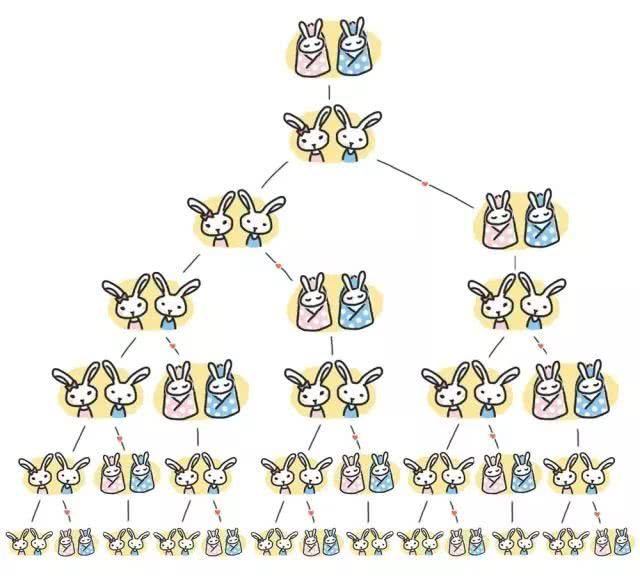
\includegraphics[scale=0.45]{img/Chapter4/4-4/1.png}
\end{figure}

\begin{lstlisting}[language=Java]
import java.util.Scanner;

public class Fibonacci {
    public static void main(String[] args) {
        Scanner scanner = new Scanner(System.in);
        int n;
        int num1, num2, val;
        
        System.out.print("输入斐波那契数列长度:");
        n = scanner.nextInt();
        
        if(n == 1) {
            System.out.println("1");
        } else if(n == 2) {
            System.out.println("1, 1");
        } else {
            num1 = 1;
            num2 = 1;
            System.out.print("1, 1");
            for(int i = 3; i <= n; i++) {
                val = num1 + num2;
                System.out.print(", " + val);
                num1 = num2;
                num2 = val;
            }
            System.out.println();
        }
        scanner.close();
    }
}
\end{lstlisting}

\begin{tcolorbox}
    \mybox{运行结果}
    \begin{verbatim}
输入斐波那契数列长度:10
1, 1, 2, 3, 5, 8, 13, 21, 34, 55
\end{verbatim}
\end{tcolorbox}

\vspace{0.5cm}

\subsection{嵌套循环}

循环也可以进行嵌套使用。\\

\mybox{九九乘法表}\\

\begin{table}[H]
    \centering
    \setlength{\tabcolsep}{1.5mm}{
        \begin{tabular}{|c|c|c|c|c|c|c|c|c|}
            \hline
            1*1=1 & 1*2=2  & 1*3=3  & 1*4=4  & 1*5=5  & 1*6=6  & 1*7=7  & 1*8=8  & 1*9=9  \\
            \hline
            2*1=2 & 2*2=4  & 2*3=6  & 2*4=8  & 2*5=10 & 2*6=12 & 2*7=14 & 2*8=16 & 2*9=18 \\
            \hline
            3*1=3 & 3*2=6  & 3*3=9  & 3*4=12 & 3*5=15 & 3*6=18 & 3*7=21 & 3*8=24 & 3*9=27 \\
            \hline
            4*1=4 & 4*2=8  & 4*3=12 & 4*4=16 & 4*5=20 & 4*6=24 & 4*7=28 & 4*8=32 & 4*9=36 \\
            \hline
            5*1=5 & 5*2=10 & 5*3=15 & 5*4=20 & 5*5=25 & 5*6=30 & 5*7=35 & 5*8=40 & 5*9=45 \\
            \hline
            6*1=6 & 6*2=12 & 6*3=18 & 6*4=24 & 6*5=30 & 6*6=36 & 6*7=42 & 6*8=48 & 6*9=54 \\
            \hline
            7*1=7 & 7*2=14 & 7*3=21 & 7*4=28 & 7*5=35 & 7*6=42 & 7*7=49 & 7*8=56 & 7*9=63 \\
            \hline
            8*1=8 & 8*2=16 & 8*3=24 & 8*4=32 & 8*5=40 & 8*6=48 & 8*7=56 & 8*8=64 & 8*9=72 \\
            \hline
            9*1=9 & 9*2=18 & 9*3=27 & 9*4=36 & 9*5=45 & 9*6=54 & 9*7=63 & 9*8=72 & 9*9=81 \\
            \hline
        \end{tabular}
    }
    \caption{九九乘法表}
\end{table}

\begin{lstlisting}[language=Java]
public class MultiplicationTable {
    public static void main(String[] args) {
        for(int i = 1; i <= 9; i++) {
            for(int j = 1; j <= 9; j++) {
                System.out.print(
                    String.format("%d*%d=%d\t", i, j, i*j)
                );
            }
            System.out.println();
        }
    }
}
\end{lstlisting}

\vspace{0.5cm}

\mybox{输出图案}

\begin{lstlisting}
*
**
***
****
*****
\end{lstlisting}

\begin{lstlisting}[language=Java]
public class Stars {
    public static void main(String[] args) {
        for(int i = 1; i <= 5; i++) {
            for(int j = 1; j <= i; j++) {
                System.out.print("*");
            }
            System.out.println();
        }
    }
}
\end{lstlisting}

\newpage

\section{break or continue?}

\subsection{循环控制}

循环控制语句的作用是控制当前的循环结构是否继续向下执行,如果不进行控制,那么会根据既定的结构重复执行。如果有一些特殊的情况导致循环的执行中断,就称为循环的控制语句。循环控制语句的关键字有break和continue。\\

break的作用是跳出当前循环,执行当前循环之后的语句。break只能跳出一层循环,如果是嵌套循环,那么需要按照嵌套的层次,逐步使用break来跳出。break语句只能在循环体内和switch语句内使用。\\

continue的作用是跳过本轮循环,开始下一轮循环的条件判断。continue终止当前轮的循环过程,但它并不跳出循环。\\

\mybox{break}

\begin{lstlisting}[language=Java]
public class Break {
    public static void main(String[] args) {
        for(int i = 1; i <= 10; i++) {
            if(i == 5) {
                break;
            }
            System.out.print(i + " ");
        }
    }
}
\end{lstlisting}

\begin{tcolorbox}
    \mybox{运行结果}
    \begin{verbatim}
1 2 3 4
\end{verbatim}
\end{tcolorbox}

\vspace{0.5cm}

\mybox{continue}

\begin{lstlisting}[language=Java]
public class Continue {
    public static void main(String[] args) {
        for(int i = 1; i <= 10; i++) {
            if(i == 5) {
                continue;
            }
            System.out.print(i + " ");
        }
    }
}
\end{lstlisting}

\begin{tcolorbox}
    \mybox{运行结果}
    \begin{verbatim}
1 2 3 4 6 7 8 9 10
\end{verbatim}
\end{tcolorbox}

\newpage

\end{document}